\chapter{Literature Review}\label{ch:literature-review}

Systems of twinned systems represent the convergence of system of systems and digital twins. While SoS research emphasizes the orchestration of independent, heterogeneous systems to achieve collective goals \cite{maier1998architecting}, DTs focus on establishing a synchronized digital representation of physical assets. This enables real-time monitoring, analysis, and control \cite{kritzinger2018digital, tao2018digital}. Integrating these ideas creates opportunities to extend both. DTs gain scalability and coordination across multiple interacting systems, while SoS benefit from intelligent, data-driven representations of their constituents.

In a SoTS, each constituent system is augmented with one or more digital twins that provide predictive, diagnostic, and prescriptive capabilities. These DT-enhanced constituents interoperate within a larger SoS enabling higher-level coordination, adaptation, and optimization across domains. This integration supports emergent capabilities, such as federated simulation, collaborative prediction, and coordinated decision-making under uncertainty, that neither standalone DTs nor traditional SoS can achieve alone. As cyber-physical infrastructures grow in complexity, the SoTS vision has gained traction as a means to enhance reliability, interoperability, and adaptability. Recent research shows that combining DTs and SoS improves cross-system optimization and situational awareness in areas such as manufacturing, transportation, and critical infrastructure management \cite{david2024infonomics, ferreira2024framework}, positioning SoTS as a scalable and adaptive evolution of both paradigms.


To explore this convergence, a systematic study was conducted to identify, classify, and analyze works in SoTS research. 
This review aimed to achieve answer the following objectives:


\noindent \textbf{Conceptual Motivation and Integration.} 
\begin{itemize}
    \item Why are DT and SoS combined?
    \item How are DT and Sos combined?
\end{itemize}
    These questions investigate the motivations, domains, and architectures that drive SoTS development, as well as the organizational and technical mechanisms by which these systems are composed.

\noindent \textbf{Technical Characterization.}
\begin{itemize}
    \item What are the defining features of DTs within SoTS?
    \item What are the defining features of SoS within SoTS?
\end{itemize}
    These questions examine autonomy, data exchange, modelling formalisms, and emergent behaviours across constituent systems.

\noindent \textbf{Reliability, Maturity, and Implementation.}  
\begin{itemize}
    \item How are non-functional properties such as reliability and security addressed in SoTS
    \item What is the current level of research and technical maturity?
    \item What technologies and platforms are most frequently used?
\end{itemize}
These questions examine the treatment of non-functional qualities throughout the SoTS lifecycle, the current state of technological readiness, and the practical means through which such systems are engineered and deployed.


Together, these all these research questions guided the extraction of key patterns, challenges, and design practices observed in existing SoTS literature.  

The study followed a systematic protocol consistent with the guidelines of \cite{kitchenham2007guidelines} and \cite{wohlin2020guidelines}, comprising the following phases:

\begin{enumerate}
    \item Database Search and Screening: A comprehensive search across Scopus, Web of Science, IEEE Xplore, and ACM Digital Library, returning an initial corpus of 317 studies.
    \item Selection and Quality Assessment: Application of explicit inclusion and exclusion criteria, duplicate removal, and quality evaluation
    \item Snowballing and Validation: Forward and backward snowballing added relevant works, resulting in a final set of 80 high-quality primary studies.
\end{enumerate}



\section{Study Design}
\label{sec:literature-review-study-design}
a systematic literature review was conducted following the established guidelines of \cite{kitchenham2007guidelines} and \cite{wohlin2020guidelines}. 
The review process was designed to capture both the conceptual and technical aspects of SoTS, focusing on how digital twin and system of systems principles are integrated, implemented, and evaluated in the literature.

\begin{figure}[H]
\centering
\fbox{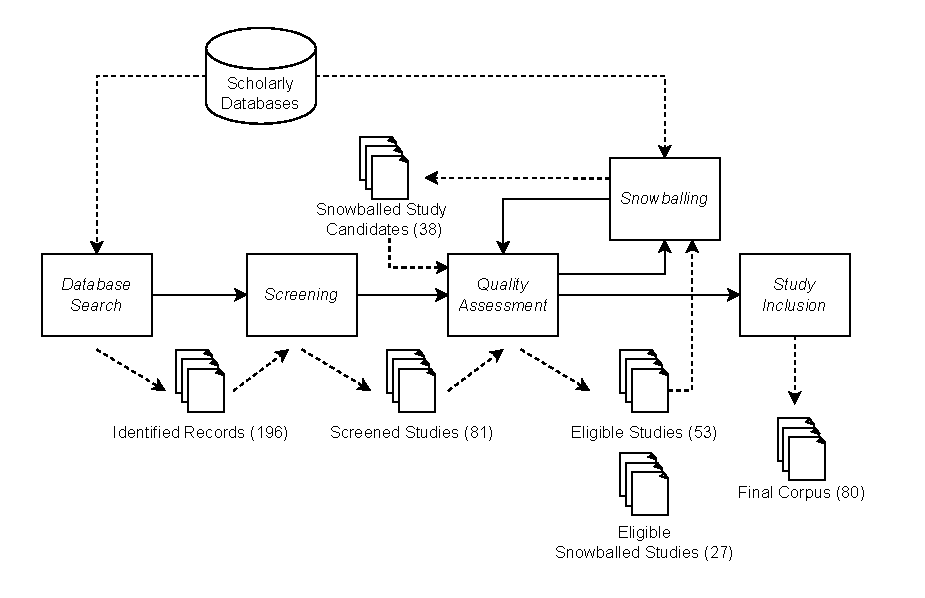
\includegraphics[width=\textwidth]{figures/Literature Review/Study Design Diagram.drawio.pdf}}
\caption{Overview of the study design and selection workflow used for the SoTS systematic literature review.}
\label{fig:literature_review_study_design_overview}
\end{figure}

The study was conducted in four main phases, as illustrated in Figure~\ref{fig:literature_review_study_design_overview}:

\begin{enumerate}
    \item \textbf{Planning and Scope Definition:}  
    The review was structured around the research questions introduced in Section~\ref{chapter:literature-review}, which investigate the motivations, architectures, reliability concerns, maturity, and technological underpinnings of SoTS.  
    A search protocol and quality assessment strategy were developed prior to data collection to ensure transparency and repeatability.

    \item \textbf{Database Search and Screening:}  
    A structured query was executed across four major indexing databases—\textit{Scopus}, \textit{Web of Science}, \textit{IEEE Xplore}, and \textit{ACM Digital Library}.  
    Searches were limited to peer-reviewed publications within Computer Science and Engineering disciplines, and included synonymous expressions for SoTS such as “aggregated digital twins,” “system of digital twins,” and “digital twin of systems.”

    \item \textbf{Selection and Quality Assessment:}  
    The initial corpus was screened through automated and manual filtering to remove duplicates and out-of-scope papers.  
    Each remaining study was independently assessed by two reviewers against predefined exclusion criteria (e.g., relevance, completeness, and clarity of SoS/DT descriptions).  
    Inter-rater agreement and Cohen’s~\(\kappa\) were computed to verify the consistency of inclusion decisions.

    \item \textbf{Data Extraction and Synthesis:}  
    Data were extracted using a structured coding framework, focusing on: (1) conceptual alignment between DT and SoS principles, (2) system architectures and modelling approaches, (3) reliability and non-functional considerations, (4) technical and research maturity, and (5) implementation technologies.  
    A combination of quantitative (frequency-based) and qualitative (content analysis) synthesis methods was used to identify recurring themes and patterns.
\end{enumerate}

\begin{table*}[]
\centering
\setlength{\tabcolsep}{1em}
\caption{Search statistics}
\label{tab:literature_review_search_statistics}
\footnotesize
\begin{tabular}{@{}lrrr@{\hspace{2pt}}lr@{}}
\toprule
\multicolumn{1}{c}{\textbf{Search round}} & \multicolumn{1}{c}{\textbf{All}} & \multicolumn{1}{c}{\textbf{Excluded}} & \multicolumn{2}{c}{\textbf{Included}} & \multicolumn{1}{c}{\textbf{Agreement}} \\ \midrule
\textbf{Automated search} & & & & & \\
\;\;\corner{} Duplicate removal & 317 & 121 & 196 &   &  \\
\;\;\corner{} E0 & 196 & 71 & 125 &   &  \\
\;\;\corner{} E1--E3 & 125 & 44 & \textbf{81} & & $IRA=0.88$ / $\kappa=0.734$ \\
\textbf{Quality assessment} & & & & & \\
\;\;\corner{} Q1 or Q2 insufficient & 81 & 22 & 59 &   &  \\
\;\;\corner{} Q3 insufficient & 59 & 6 & 53 &   &  \\
\;\;\corner{} Q4 insufficient & 53 & 0 & 53 &   &  \\
\textbf{Subtotal} & \textbf{317} & \textbf{264} & \included{53} & \textbf{(16.72\%)} & \\
\midrule
\textbf{Snowballing} & & & & & \\
\;\;\corner{} Backward & & & & & \\
\;\;\;\;\corner{} Selection by reference & 1\,666 & 1\,521 & 145 & & \\
\;\;\;\;\corner{} Selection by abstract & 145 & 132 & \textbf{13} & & \\
\;\;\corner{} Forward & 586 & 561 & \textbf{25} & &  \\
\;\;\corner{} Total abstracts screened & 731 & 693  & \textbf{38} & & $IRA=0.944$ / $\kappa=0.488$ \\
\textbf{Quality assessment} & & & & & \\
\;\;\corner{} Q1 or Q2 insufficient & 38 & 9 & 29 &   &  \\
\;\;\corner{} Q3 insufficient & 29 & 2 & 27 &   &  \\
\;\;\corner{} Q4 insufficient & 27 & 0 & \textbf{27} &  &  \\
\textbf{Subtotal} & \textbf{2\,252} & \textbf{2\,225} & \included{27} & \textbf{(1.19\%)} & \\
\midrule
\textbf{Total} & \textbf{2\,569} & \textbf{2\,489} & \included{80} & \textbf{(3.11\%)} & \\
\bottomrule
\end{tabular}
\end{table*}

The search and selection statistics are summarized in Table~\ref{tab:literature_review_search_statistics}.  
A total of 317 studies were initially retrieved, and after the application of inclusion, exclusion, and quality filters, \textbf{80 primary studies} were included in the final corpus.  
These studies collectively represent the current state of SoTS research, capturing both theoretical advances and empirical applications across diverse domains such as manufacturing, energy, and urban infrastructure.



\section{Architecture} 

\section{Results}

\subsection{Conceptual Motivation and Integration}
\subsubsection{RQ1: Why are DT and SoS combined?}
% \begin{table*}[htp]
            \centering
            \scriptsize
            \caption{Motivations for combining DT and SoS}
            \label{tab:motivations-table}
            \begin{tabular}{@{}p{4cm}l p{8.5cm}@{}}
            \toprule
            \multicolumn{1}{c}{\textbf{Motivation}} & 
            \multicolumn{1}{c}{\textbf{Frequency}} & 
            \multicolumn{1}{c}{\textbf{Studies}} \\ 
            \midrule
            Optimization & \maindatabar{30} & \cite{bao2024digital,becue2018cyberfactory,chavezbaliguat2023digital,chen2018digital,duan2023digital,folds2019digital,gill2022method,howard2021greenhouse,jirsa2024use,joseph2021aggregated,kruger2022towards,lee2022simulation,li2022cognitive,li2024comprehensive,lippi2023enabling,liu2020web-based,maheshwari2022digital,malayjerdi2022combined,novak2022digitalized,park2020digital,pickering2023towards,pillai2023digital,potteiger2023live,priyanta2024is,somma2023digital,vermesan2021internet,villalonga2021decision-making,wullink2024foundational,zhang2022multi-scale,zhang2021bi-level} \\
Integration & \maindatabar{25} & \cite{acharya2023twins,alam2017c2ps,ashtaritalkhestani2019architecture,aziz2022empowering,bellavista2023requirements,demir2023vertically-integrated,dobie2024network,doubell2023digital,esterle2021digital,gil2023modeling,gil2024integrating,gollner2022collaborative,hatledal2020co-simulation,heininger2021capturing,heithoff2023challenges,hofmeister2024cross-domain,hofmeister2024semantic,human2023design,larsen2024towards,mahoro2023articulating,monsalve2021novel,reiche2021digital,savur2019hrc-sos,stary2022privacy,vogel-heuser2021approach} \\
Validation & \maindatabar{15} & \cite{bertoni2022digital,clark2021chapter,coupaye2023graph-based,dahmen2022modeling,dickopf2019holistic,ehemann2023digital,kulkarni2019towards,marah2023architecture,mavromatis2024umbrella,oquendo2019dealing,redelinghuys2020six-layer,samak2023autodrive,schluse2017experimentable,wagner2023using,wang2024construction} \\
Maintainability & \maindatabar{10} & \cite{altamiranda2019system,barden2022academic,binder2021utilizing,hatakeyama2018systems,jiang2022novel,kutzke2021subsystem,lopez2023modeling,parri2021framework,parri2019jarvis,saraeian2022digital} \\
\bottomrule
            \end{tabular}
            \end{table*}

\subsubsection{RQ2: How are DT and Sos combined?}

\subsection{Technical Characterization.}
\subsubsection{RQ3: What are the defining features of DTs within SoTS?}
\subsubsection{RQ4: What are the defining features of SoS within SoTS?}

\subsection{Reliability, Maturity, and Implementation.}
\subsubsection{RQ5: How are non-functional properties such as reliability and security addressed in SoTS}
\subsubsection{RQ6: What is the current level of research and technical maturity?}
\subsubsection{RQ7: What technologies and platforms are most frequently used?}


\section{Discussion}

